\documentclass{beamer}

\usepackage{ngerman}
\usepackage[utf8]{inputenc}
\usepackage{graphicx}
\usepackage{url}
\usepackage{amsmath}
\usepackage{amsfonts}
\usepackage{amssymb}
\usepackage{amstext}

\title[KivS Abschlusspräsentation]{Kommunikation in verteilten Systemen\\Abschlusspräsentation der praktischen Übung}
\author{Paul Scherer, Jonas Barteldrees}
\institute[Institut für Informatik]{Universität Bonn, Institut für Informatik}
\usetheme{Berlin}

\begin{document}
\frame{
	\maketitle
}

\frame{
	\frametitle{Übersicht}
	\tableofcontents
}
\section{Datenanalyse}
	\frame{
		\frametitle{Auffälligkeiten}
		\begin{itemize}
			\item Aufteilung in diskrete Stufen
			  \begin{itemize}
			   \item ausreichende Bandbreite
			   \item Route gleichbleibend
			  \end{itemize}
			\item neuere Messungen unregelmäßig
			  \begin{itemize}
			   \item erhöhte Last
			   \item dynamischere Route
			  \end{itemize}
			\item doppelstufige Pings Ende 2015
			   \begin{itemize}
			   \item Paket auf zwei potentiellen Routen
			  \end{itemize}
		\end{itemize}
	}
\section{Bandbreitenmessung}
	\subsection{Messaufbau}
		\frame{
			\frametitle{Verfahren}
			\begin{enumerate}
			  \item Verbindung zum Informatiknetz per VPN
			  \item Herunterladen der Testdatei via Webbrowser
			  	\begin{itemize}
				  	\item linux-3.9.2.tar.xz, 68,7 MB
			  	\end{itemize}
			  \item Paketaufzeichnung mittels Wireshark
			  \item Auswertung mit Wireshark
			    \begin{itemize}
				    \item Statistics $\rightarrow$ IOGraph
			    \end{itemize}
			\end{enumerate}
		}

	\subsection{HTTP}
		\frame{
			\frametitle{graphische Auswertung: Stufen}
			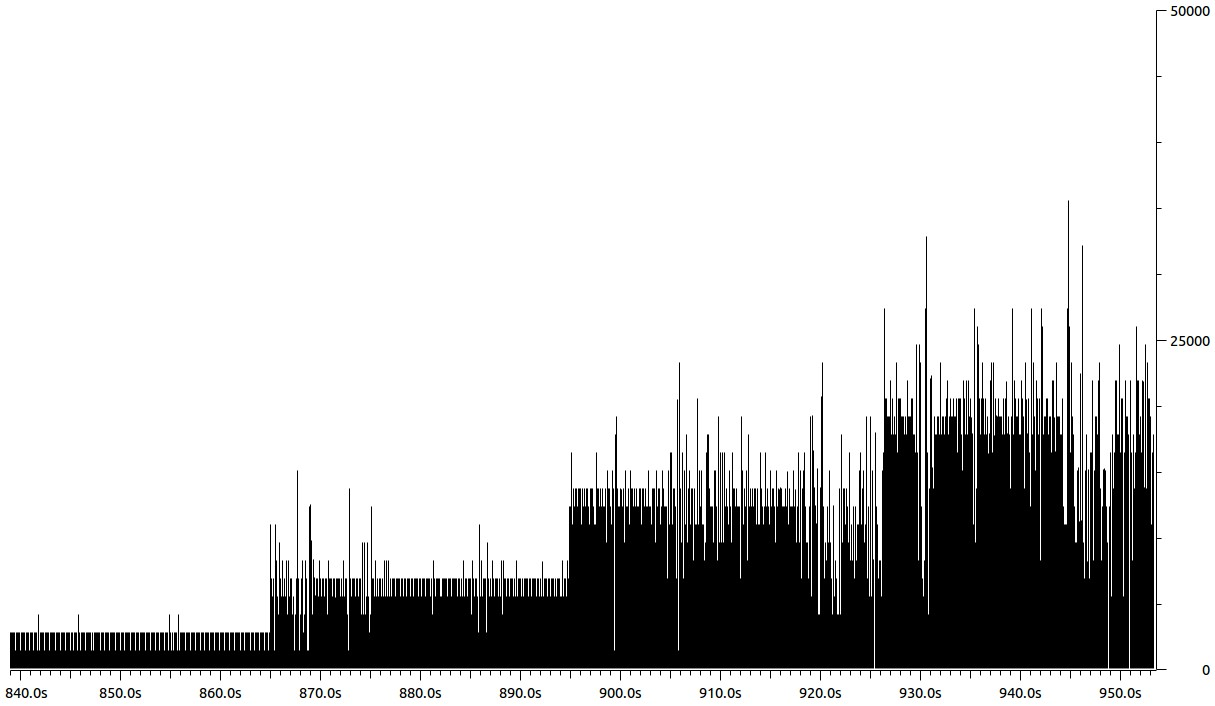
\includegraphics[scale = 0.25]{BandbreiteHTTPEDU.jpg}
		}
		
		\frame{
			\frametitle{graphische Auswertung: Bandbreitenausreißer}
			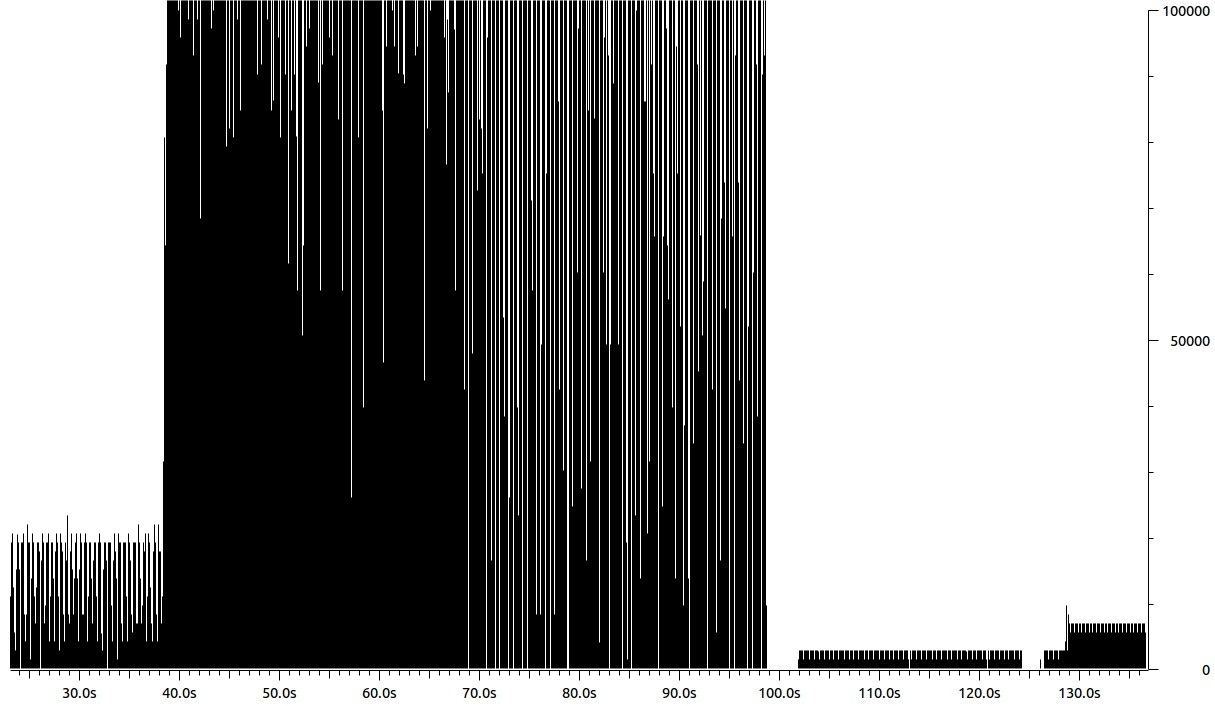
\includegraphics[scale = 0.25]{BandbreiteHTTPLAN.jpg}
		}
		
		\frame{
			\frametitle{graphische Auswertung: zeitliche Begrenzung}
			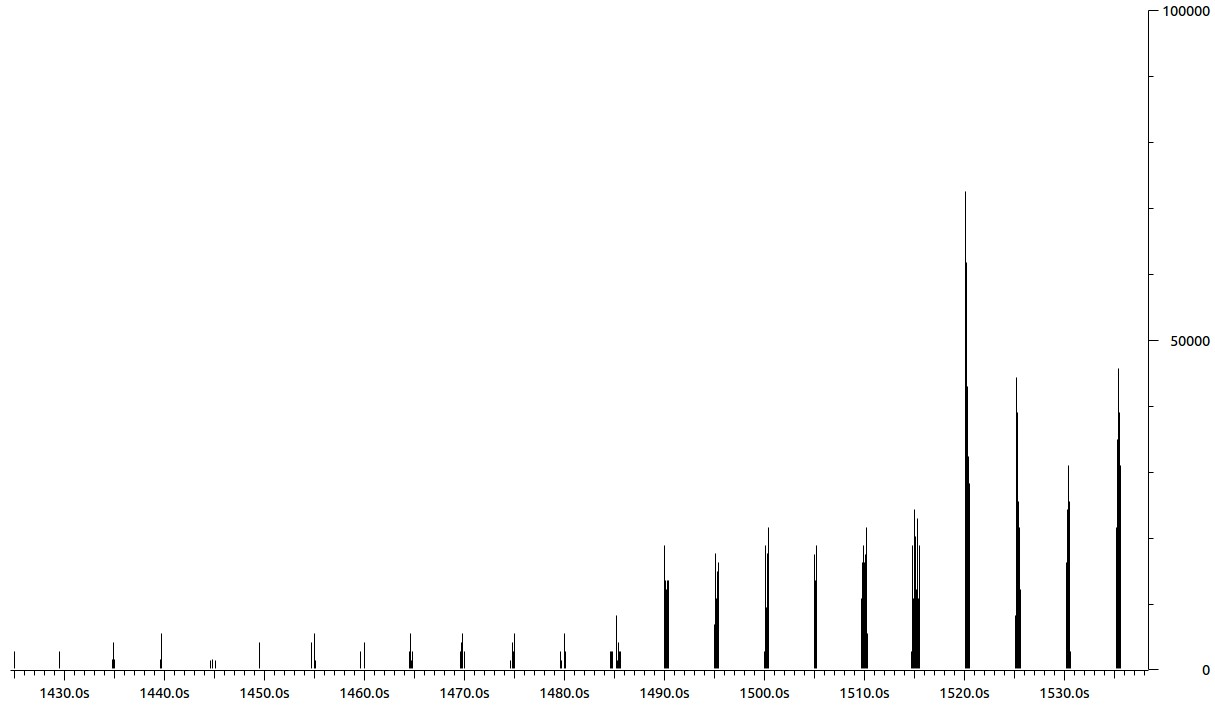
\includegraphics[scale = 0.25]{BandbreiteHTTPLAN2VPN.jpg}
		}
		
		\frame{
			\frametitle{Extrahierte Werte}
			\begin{itemize}
				\item Bandbreitenbegrenzung: 33333 $\frac{byte}{s}$, 66666 $\frac{byte}{s}$, 200000 $\frac{byte}{s}$
				\item Wechselfrequenz: 30 s, periodisch
			\end{itemize}
		}

	\subsection{FTP}
		\frame{
			\frametitle{graphische Auswertung}
			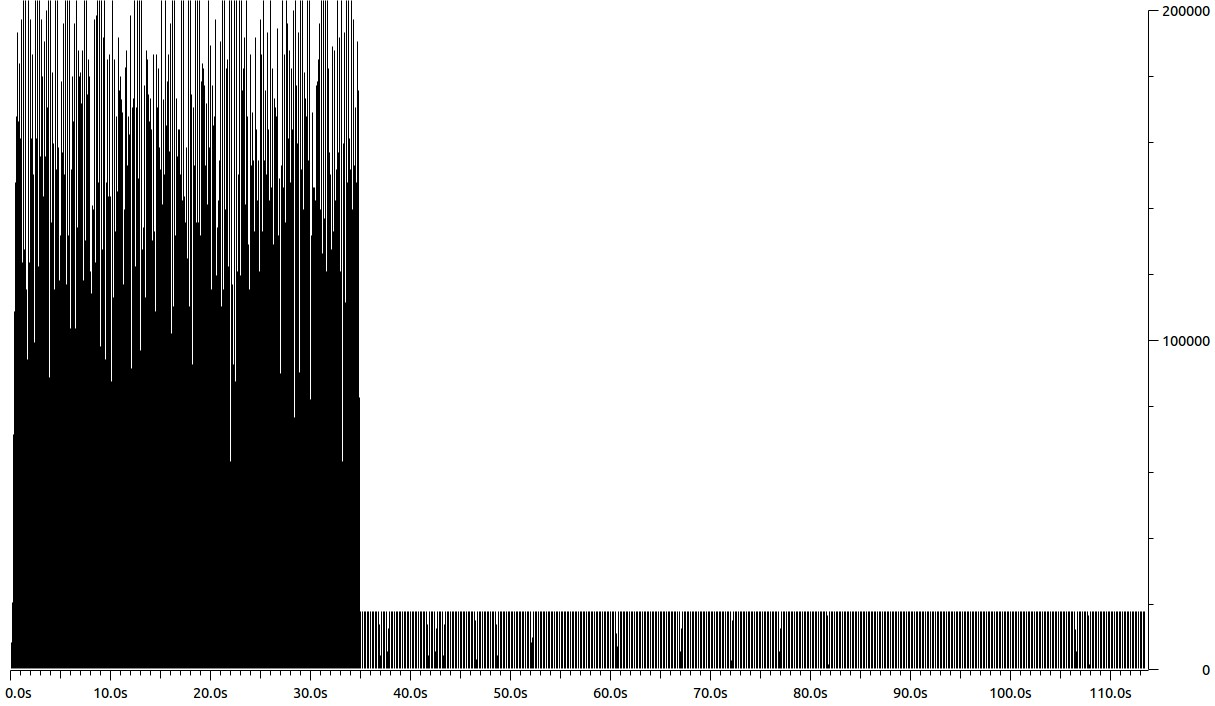
\includegraphics[scale = 0.25]{BandbreiteFTPLAN.jpg}
		}
		
		\frame{
			\frametitle{Extrahierte Werte}
			\begin{itemize}
				\item Bandbreitenbegrenzung: ca. 200000 $\frac{byte}{s}$
				\item Wechselfrequenz: nach 35 s, einmalig
			\end{itemize}
		}
\section{Anhang}
	\frame{
		\frametitle{Auswertung RTT über Ping-Nr}
		
\includegraphics[scale = 0.5]{parsedNum.jpg}
	}
	
	\frame{
		\frametitle{Auswertung RTT über Zeit}
		
\includegraphics[scale = 0.5]{parsedTime.jpg}
	}
	
	\frame{
		\frametitle{Auswertung Boxplots}
		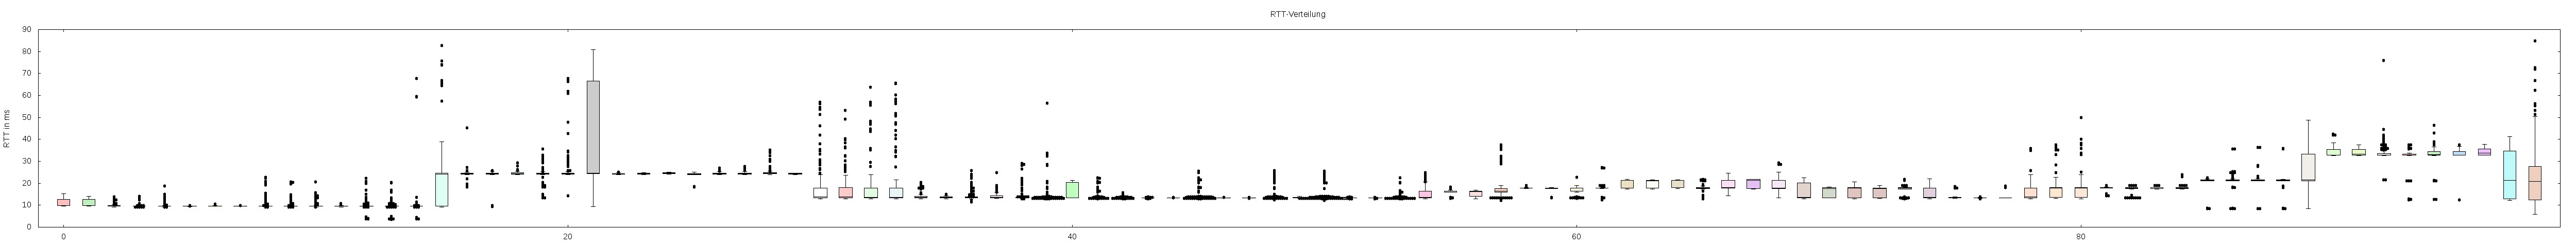
\includegraphics[scale = 0.5]{boxplot.jpg}
	}
\end{document}